\documentclass[a4paper, 11pt]{article}
\usepackage{geometry}
\geometry{letterpaper, margin=1in}
\usepackage{graphicx}
\graphicspath{ {images/} }

\usepackage{amsmath}
\usepackage{amssymb}  
\usepackage{amsthm}
\usepackage{ulem}

\usepackage{enumitem}


\usepackage{pdfpages} % for including full pdf pages

\usepackage{empheq}

\usepackage{listings}


%format to allow bolded theorems, corollaries, etc...
\newtheorem*{theorem}{Theorem}
\newtheorem*{corollary}{Corollary}
\newtheorem*{lemma}{Lemma}
\newtheorem*{definition}{Definition}
\newtheorem*{Example}{Example} 
\newtheorem*{Remark}{Remark}

% stop typing \mathbb a thousand times 
\newcommand{\R}{\mathbb{R}}
\newcommand{\C}{\mathbb{C}}
\newcommand{\F}{\mathbb{F}}
\newcommand{\E}{\mathbb{E}}
\newcommand{\sphere}{\mathbb{S}}

% commands for bra-ket notation
\newcommand{\bra}[1]{\ensuremath{\left\langle#1\right|}}
\newcommand{\ket}[1]{\ensuremath{\left|#1\right\rangle}}
\newcommand{\bracket}[2]{\ensuremath{\left\langle #1 \middle| #2 \right\rangle}}
\newcommand{\matrixel}[3]{\ensuremath{\left\langle #1 \middle| #2 \middle| #3 \right\rangle}}
\newcommand{\expectation}[1]{\ensuremath{\left\langle #1 \right\rangle}}

% vector stuff
\newcommand{\basis}[1]{\hat{\mathbf{e}}_#1}
\newcommand{\unit}[1]{\hat{\boldsymbol{#1}}}
\newcommand{\bvec}[1]{\vec{\boldsymbol{#1}}}


% change margins for solution
\newenvironment{solution}{%
	\begin{list}{}{%
			\setlength{\topsep}{0pt}%
			\setlength{\leftmargin}{0.5cm}%
			\setlength{\rightmargin}{0.5cm}%
			\setlength{\listparindent}{\parindent}%
			\setlength{\itemindent}{\parindent}%
			\setlength{\parsep}{\parskip}%
		}%
		\item[]}{\end{list}}



\begin{document}
\noindent
\large\textbf{Assignment 2: Design} \hfill \textbf{John Waczak} \\
\normalsize CS 162 \hfill  Date: \today 
\par\noindent\rule{\textwidth}{0.4pt} \\\\



\section*{Understanding the problem}

\textit{In your own words, explain what YOU think the problem is asking you to
  do.  Document your uncertainties about the problem and anything else that you
  feel was unclear or vague}\\

The problem is asking us to design a program for a pizza restaurant which will
present different functionality depending on whether a customer or employee
chooses to use it. Employees must first login to the system and have their id
and password checked against data in a separate file. After the user identifies
themselves as employee or customer, they are then presented with options to view
the menu, place orders, add menu items, etc... Some of these options are
exclusive to either the employee or the customer. The user may also may logout
and return to the welcome screen at any time. After making a choice, the user is
then redirected to the prompt menu for further options until they decide to
logout and then quit the program. 
\section*{Devising a plane/design}

\textit{Provide an algorithm/pseudo code to help solve the problem. In addition,
  draw pictures/flow charts to help you devise your plan, as well as any other
  design decisions you make, such as how to manage your time, how to decompose
  the problem, where to start first, etc. }\\ 

See flowchart on next page

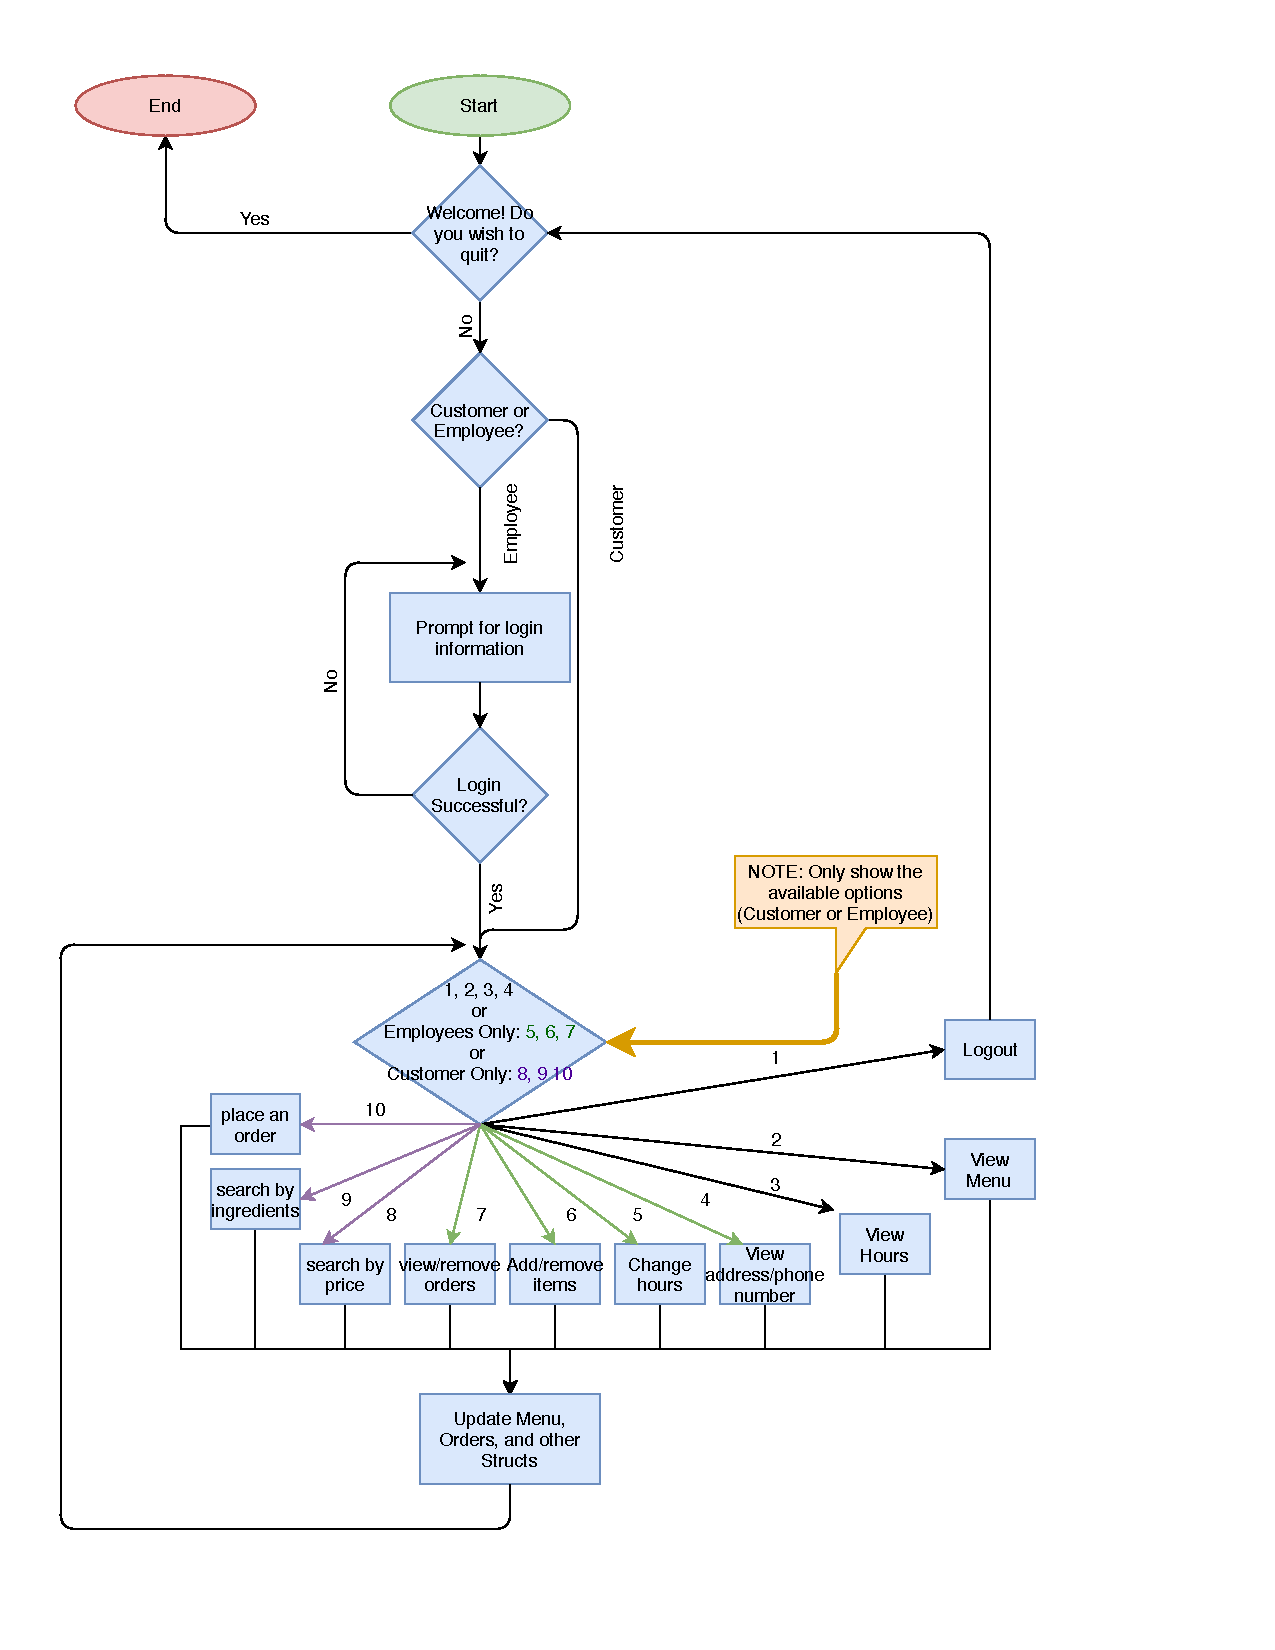
\includepdf{images/flow_chart.pdf}


\section*{Looking back / testing}

\textit{This includes any checking/self-reflection you did while solving the
  problem, which includes using a calculator to make sure the output is correct,
  testing to make sure your code executes correctly and behaves the way you
  expect under specific circumstances, using sources of information to make
  sense of the results, etc. However, you need to think about the input prior to
  implementation!!!}\\
\vspace{5em}

\begin{center}
 \begin{tabular}{l|r} % <-- Alignments: 1st column left, 2nd middle and 3rd right, with vertical lines in between
   \textbf{Input} & \textbf{Expected} \\
    &    \\
   \hline
   Incorrect id: asdflj;lkj & could not find login information. please try again   \\
   Incorrect pass: asdfasdfas & Password does not match our records: Please try again  \\
   Incorrect pass (x3) & You failed to log in. (Quit program)   \\
   Choose an option: 1  &Return to welcome screen  \\
   Choose an option: 2 & Print out the menu  \\
   Choose an option: 3 & Print out hours of service  \\
   Choose an option: 4 & Prompt for address or phone number  \\
   Choose an option: 5 & Prompt for open and close times  \\
   Choose an option: 6 & Prompt: Would you like to add or remove menu items? \\
   Choose an option: 7 & Prompt: Would like like to view or remove orders?  \\
   Choose an option: 8 & Prompt: Please enter the maximum amount you wish to spend (\$)  \\
   Choose an option: 9 & Prompt: Please enter an ingredient to search by.  \\
   Choose an option: 10 & Prompt: Please enter the name of the pizza you would like to order.  \\
 \end{tabular}
\end{center} 






\end{document}





































